\resizebox{\linewidth}{!}{
\begin{tikzpicture}
    % Colors definition
    \pgfdeclaredecoration{single pulse}{initial}{
    \state{initial}[width=\pgfdecoratedinputsegmentlength]
    {%
        % Initial Line
        \pgfpathlineto{\pgfpoint{0.1*\pgfdecoratedinputsegmentlength}{0mm}}%    
        % P Peak
        \pgfpathsine{\pgfpoint{0.2\pgfdecorationsegmentlength}{0.15\pgfdecorationsegmentamplitude}}%
        \pgfpathcosine{\pgfpoint{0.2\pgfdecorationsegmentlength}{-0.15\pgfdecorationsegmentamplitude}}%
        % P - Q Line
        \pgfpathlineto{\pgfpoint{0.6\pgfdecorationsegmentamplitude}{0mm}}%
        % Q Valley
        \pgfpathsine{\pgfpoint{0.1\pgfdecorationsegmentlength}{-0.15\pgfdecorationsegmentamplitude}}
        \pgfpathcosine{\pgfpoint{0.01\pgfdecorationsegmentlength}{0.15\pgfdecorationsegmentamplitude}}%
        % R Peak
        \pgfpathsine{\pgfpoint{0.15\pgfdecorationsegmentlength}{\pgfdecorationsegmentamplitude}}%
        \pgfpathcosine{\pgfpoint{0.15\pgfdecorationsegmentlength}{-\pgfdecorationsegmentamplitude}}%
        % S Valley
        \pgfpathsine{\pgfpoint{0.15\pgfdecorationsegmentlength}{-0.5\pgfdecorationsegmentamplitude}}
        \pgfpathcosine{\pgfpoint{0.15\pgfdecorationsegmentlength}{0.5\pgfdecorationsegmentamplitude}}%
        % S to T line
        \pgfpathlineto{\pgfpoint{1.25\pgfdecorationsegmentamplitude}{0mm}}%
        % T Peak
        \pgfpathsine{\pgfpoint{0.8\pgfdecorationsegmentlength}{0.3\pgfdecorationsegmentamplitude}}%
        \pgfpathcosine{\pgfpoint{0.8\pgfdecorationsegmentlength}{-0.3\pgfdecorationsegmentamplitude}}%
        % Last Line
        \pgfpathlineto{\pgfpointdecoratedinputsegmentlast}%
    }
    \state{final}{}%
    }

    \fill[gray!10, draw=black] (-0.75, -0.75) rectangle (6.25, 1.75);
    \node at (-0.5, -0.5) {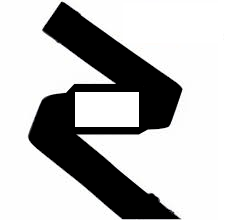
\includegraphics[width=10pt]{img/hrband.png}};
    %\node at (5.5, 1.5) {\textbf{\small{Sensor}}};

    \draw[->, dashed] (5.55,0) -- (6,0) node[pos=.5, anchor=north, xshift=-10pt] {\tiny{Time ($s$)}};
    \draw[->, dashed] (0,0) -- (0,1.25) node[anchor=south, xshift=10pt] {\tiny{Amplitude ($mV$)}};
    \draw[decoration={single pulse,amplitude=8mm,segment length=2mm},decorate] (0,0) -- (2,0);
    \draw[decoration={single pulse,amplitude=8mm,segment length=2mm},decorate] (2,0) -- (4,0);
    \draw[decoration={single pulse,amplitude=6mm,segment length=2mm},decorate] (4,0) -- (5.5,0);
    \draw[<->, dashed, thick] (0.55, 0.7) -- (2.5, 0.7);
    \draw[<->, dashed, thick] (2.55, 0.55) -- (4.35, 0.55);
    \node[align=center] at (0.5, 0.95) {\tiny{$\text{R}_0$}};
    \node[align=center] at (2.2, 0.3) {\tiny{$\text{P}_1$}};
    \node[align=center] at (2.4, -0.2) {\tiny{$\text{Q}_1$}};
    \node[align=center] at (2.7, -0.55) {\tiny{$\text{S}_1$}};
    \node[align=center] at (3.15, 0.38) {\tiny{$\text{T}_1$}};
    \node[align=center] at (2.5, 0.95) {\tiny{$\text{R}_1$}};
    \node[align=center] at (4.25, 0.8) {\tiny{$\text{R}_2$}};

    % Signal
    \fill[black] (6.5, 0) circle (0.05);
    \draw (6.75, -0.15) arc (-20:20:0.5);
    \draw (6.95, -0.25) arc (-30:30:0.5);
    \draw (7.15, -0.35) arc (-40:40:0.5);

    % Data file
    \node[align=center] at (9, 1.2) {\tiny{\textbf{\texttt{gateway://data/data\_file.csv}}}};
    \draw (7.45, -0.75) -- (7.45, 1) -- (10.5,1) -- (10.5, -0.5) to[out=180, in=0] (7.45, -0.75);
    \node[align=center] at (9, 0.2) {\tiny{\texttt{t}$\left(\text{R}_1\right)$, \xspace\texttt{t}$\left(\text{R}_1\right)$ - \texttt{t}$\left(\text{R}_0\right)$} \\ \tiny{\texttt{t}$\left(\text{R}_2\right)$, \xspace\texttt{t}$\left(\text{R}_2\right)$ - \texttt{t}$\left(\text{R}_1\right)$} \\ \tiny{\textbf{$\vdots$}}};
\end{tikzpicture}}
